% Options for packages loaded elsewhere
\PassOptionsToPackage{unicode}{hyperref}
\PassOptionsToPackage{hyphens}{url}
\PassOptionsToPackage{dvipsnames,svgnames,x11names}{xcolor}
%
\documentclass[
  letterpaper,
  DIV=11,
  numbers=noendperiod]{scrartcl}

\usepackage{amsmath,amssymb}
\usepackage{lmodern}
\usepackage{iftex}
\ifPDFTeX
  \usepackage[T1]{fontenc}
  \usepackage[utf8]{inputenc}
  \usepackage{textcomp} % provide euro and other symbols
\else % if luatex or xetex
  \usepackage{unicode-math}
  \defaultfontfeatures{Scale=MatchLowercase}
  \defaultfontfeatures[\rmfamily]{Ligatures=TeX,Scale=1}
\fi
% Use upquote if available, for straight quotes in verbatim environments
\IfFileExists{upquote.sty}{\usepackage{upquote}}{}
\IfFileExists{microtype.sty}{% use microtype if available
  \usepackage[]{microtype}
  \UseMicrotypeSet[protrusion]{basicmath} % disable protrusion for tt fonts
}{}
\makeatletter
\@ifundefined{KOMAClassName}{% if non-KOMA class
  \IfFileExists{parskip.sty}{%
    \usepackage{parskip}
  }{% else
    \setlength{\parindent}{0pt}
    \setlength{\parskip}{6pt plus 2pt minus 1pt}}
}{% if KOMA class
  \KOMAoptions{parskip=half}}
\makeatother
\usepackage{xcolor}
\setlength{\emergencystretch}{3em} % prevent overfull lines
\setcounter{secnumdepth}{-\maxdimen} % remove section numbering
% Make \paragraph and \subparagraph free-standing
\ifx\paragraph\undefined\else
  \let\oldparagraph\paragraph
  \renewcommand{\paragraph}[1]{\oldparagraph{#1}\mbox{}}
\fi
\ifx\subparagraph\undefined\else
  \let\oldsubparagraph\subparagraph
  \renewcommand{\subparagraph}[1]{\oldsubparagraph{#1}\mbox{}}
\fi

\usepackage{color}
\usepackage{fancyvrb}
\newcommand{\VerbBar}{|}
\newcommand{\VERB}{\Verb[commandchars=\\\{\}]}
\DefineVerbatimEnvironment{Highlighting}{Verbatim}{commandchars=\\\{\}}
% Add ',fontsize=\small' for more characters per line
\usepackage{framed}
\definecolor{shadecolor}{RGB}{241,243,245}
\newenvironment{Shaded}{\begin{snugshade}}{\end{snugshade}}
\newcommand{\AlertTok}[1]{\textcolor[rgb]{0.68,0.00,0.00}{#1}}
\newcommand{\AnnotationTok}[1]{\textcolor[rgb]{0.37,0.37,0.37}{#1}}
\newcommand{\AttributeTok}[1]{\textcolor[rgb]{0.40,0.45,0.13}{#1}}
\newcommand{\BaseNTok}[1]{\textcolor[rgb]{0.68,0.00,0.00}{#1}}
\newcommand{\BuiltInTok}[1]{\textcolor[rgb]{0.00,0.23,0.31}{#1}}
\newcommand{\CharTok}[1]{\textcolor[rgb]{0.13,0.47,0.30}{#1}}
\newcommand{\CommentTok}[1]{\textcolor[rgb]{0.37,0.37,0.37}{#1}}
\newcommand{\CommentVarTok}[1]{\textcolor[rgb]{0.37,0.37,0.37}{\textit{#1}}}
\newcommand{\ConstantTok}[1]{\textcolor[rgb]{0.56,0.35,0.01}{#1}}
\newcommand{\ControlFlowTok}[1]{\textcolor[rgb]{0.00,0.23,0.31}{#1}}
\newcommand{\DataTypeTok}[1]{\textcolor[rgb]{0.68,0.00,0.00}{#1}}
\newcommand{\DecValTok}[1]{\textcolor[rgb]{0.68,0.00,0.00}{#1}}
\newcommand{\DocumentationTok}[1]{\textcolor[rgb]{0.37,0.37,0.37}{\textit{#1}}}
\newcommand{\ErrorTok}[1]{\textcolor[rgb]{0.68,0.00,0.00}{#1}}
\newcommand{\ExtensionTok}[1]{\textcolor[rgb]{0.00,0.23,0.31}{#1}}
\newcommand{\FloatTok}[1]{\textcolor[rgb]{0.68,0.00,0.00}{#1}}
\newcommand{\FunctionTok}[1]{\textcolor[rgb]{0.28,0.35,0.67}{#1}}
\newcommand{\ImportTok}[1]{\textcolor[rgb]{0.00,0.46,0.62}{#1}}
\newcommand{\InformationTok}[1]{\textcolor[rgb]{0.37,0.37,0.37}{#1}}
\newcommand{\KeywordTok}[1]{\textcolor[rgb]{0.00,0.23,0.31}{#1}}
\newcommand{\NormalTok}[1]{\textcolor[rgb]{0.00,0.23,0.31}{#1}}
\newcommand{\OperatorTok}[1]{\textcolor[rgb]{0.37,0.37,0.37}{#1}}
\newcommand{\OtherTok}[1]{\textcolor[rgb]{0.00,0.23,0.31}{#1}}
\newcommand{\PreprocessorTok}[1]{\textcolor[rgb]{0.68,0.00,0.00}{#1}}
\newcommand{\RegionMarkerTok}[1]{\textcolor[rgb]{0.00,0.23,0.31}{#1}}
\newcommand{\SpecialCharTok}[1]{\textcolor[rgb]{0.37,0.37,0.37}{#1}}
\newcommand{\SpecialStringTok}[1]{\textcolor[rgb]{0.13,0.47,0.30}{#1}}
\newcommand{\StringTok}[1]{\textcolor[rgb]{0.13,0.47,0.30}{#1}}
\newcommand{\VariableTok}[1]{\textcolor[rgb]{0.07,0.07,0.07}{#1}}
\newcommand{\VerbatimStringTok}[1]{\textcolor[rgb]{0.13,0.47,0.30}{#1}}
\newcommand{\WarningTok}[1]{\textcolor[rgb]{0.37,0.37,0.37}{\textit{#1}}}

\providecommand{\tightlist}{%
  \setlength{\itemsep}{0pt}\setlength{\parskip}{0pt}}\usepackage{longtable,booktabs,array}
\usepackage{calc} % for calculating minipage widths
% Correct order of tables after \paragraph or \subparagraph
\usepackage{etoolbox}
\makeatletter
\patchcmd\longtable{\par}{\if@noskipsec\mbox{}\fi\par}{}{}
\makeatother
% Allow footnotes in longtable head/foot
\IfFileExists{footnotehyper.sty}{\usepackage{footnotehyper}}{\usepackage{footnote}}
\makesavenoteenv{longtable}
\usepackage{graphicx}
\makeatletter
\def\maxwidth{\ifdim\Gin@nat@width>\linewidth\linewidth\else\Gin@nat@width\fi}
\def\maxheight{\ifdim\Gin@nat@height>\textheight\textheight\else\Gin@nat@height\fi}
\makeatother
% Scale images if necessary, so that they will not overflow the page
% margins by default, and it is still possible to overwrite the defaults
% using explicit options in \includegraphics[width, height, ...]{}
\setkeys{Gin}{width=\maxwidth,height=\maxheight,keepaspectratio}
% Set default figure placement to htbp
\makeatletter
\def\fps@figure{htbp}
\makeatother

\KOMAoption{captions}{tableheading}
\makeatletter
\makeatother
\makeatletter
\makeatother
\makeatletter
\@ifpackageloaded{caption}{}{\usepackage{caption}}
\AtBeginDocument{%
\ifdefined\contentsname
  \renewcommand*\contentsname{Table of contents}
\else
  \newcommand\contentsname{Table of contents}
\fi
\ifdefined\listfigurename
  \renewcommand*\listfigurename{List of Figures}
\else
  \newcommand\listfigurename{List of Figures}
\fi
\ifdefined\listtablename
  \renewcommand*\listtablename{List of Tables}
\else
  \newcommand\listtablename{List of Tables}
\fi
\ifdefined\figurename
  \renewcommand*\figurename{Figure}
\else
  \newcommand\figurename{Figure}
\fi
\ifdefined\tablename
  \renewcommand*\tablename{Table}
\else
  \newcommand\tablename{Table}
\fi
}
\@ifpackageloaded{float}{}{\usepackage{float}}
\floatstyle{ruled}
\@ifundefined{c@chapter}{\newfloat{codelisting}{h}{lop}}{\newfloat{codelisting}{h}{lop}[chapter]}
\floatname{codelisting}{Listing}
\newcommand*\listoflistings{\listof{codelisting}{List of Listings}}
\makeatother
\makeatletter
\@ifpackageloaded{caption}{}{\usepackage{caption}}
\@ifpackageloaded{subcaption}{}{\usepackage{subcaption}}
\makeatother
\makeatletter
\@ifpackageloaded{tcolorbox}{}{\usepackage[many]{tcolorbox}}
\makeatother
\makeatletter
\@ifundefined{shadecolor}{\definecolor{shadecolor}{rgb}{.97, .97, .97}}
\makeatother
\makeatletter
\makeatother
\ifLuaTeX
  \usepackage{selnolig}  % disable illegal ligatures
\fi
\IfFileExists{bookmark.sty}{\usepackage{bookmark}}{\usepackage{hyperref}}
\IfFileExists{xurl.sty}{\usepackage{xurl}}{} % add URL line breaks if available
\urlstyle{same} % disable monospaced font for URLs
\hypersetup{
  pdftitle={Class 13: RNA-Seq Analysis Mini-Project},
  pdfauthor={Eric jordahl},
  colorlinks=true,
  linkcolor={blue},
  filecolor={Maroon},
  citecolor={Blue},
  urlcolor={Blue},
  pdfcreator={LaTeX via pandoc}}

\title{Class 13: RNA-Seq Analysis Mini-Project}
\author{Eric jordahl}
\date{2022-11-09}

\begin{document}
\maketitle
\ifdefined\Shaded\renewenvironment{Shaded}{\begin{tcolorbox}[boxrule=0pt, breakable, sharp corners, interior hidden, borderline west={3pt}{0pt}{shadecolor}, frame hidden, enhanced]}{\end{tcolorbox}}\fi

\hypertarget{section-1-differential-expression-analysis}{%
\section{Section 1: Differential Expression
Analysis}\label{section-1-differential-expression-analysis}}

\begin{Shaded}
\begin{Highlighting}[]
\FunctionTok{library}\NormalTok{(DESeq2)}
\NormalTok{metaFile }\OtherTok{\textless{}{-}} \StringTok{"GSE37704\_metadata.csv"}
\NormalTok{countFile }\OtherTok{\textless{}{-}} \StringTok{"GSE37704\_featurecounts.csv"}

\CommentTok{\# Import metadata and take a peak}
\NormalTok{colData }\OtherTok{=} \FunctionTok{read.csv}\NormalTok{(metaFile, }\AttributeTok{row.names=}\DecValTok{1}\NormalTok{)}
\FunctionTok{head}\NormalTok{(colData)}
\end{Highlighting}
\end{Shaded}

\begin{verbatim}
              condition
SRR493366 control_sirna
SRR493367 control_sirna
SRR493368 control_sirna
SRR493369      hoxa1_kd
SRR493370      hoxa1_kd
SRR493371      hoxa1_kd
\end{verbatim}

\begin{Shaded}
\begin{Highlighting}[]
\CommentTok{\# Import countdata}
\NormalTok{countData }\OtherTok{=} \FunctionTok{read.csv}\NormalTok{(countFile, }\AttributeTok{row.names=}\DecValTok{1}\NormalTok{)}
\FunctionTok{head}\NormalTok{(countData)}
\end{Highlighting}
\end{Shaded}

\begin{verbatim}
                length SRR493366 SRR493367 SRR493368 SRR493369 SRR493370
ENSG00000186092    918         0         0         0         0         0
ENSG00000279928    718         0         0         0         0         0
ENSG00000279457   1982        23        28        29        29        28
ENSG00000278566    939         0         0         0         0         0
ENSG00000273547    939         0         0         0         0         0
ENSG00000187634   3214       124       123       205       207       212
                SRR493371
ENSG00000186092         0
ENSG00000279928         0
ENSG00000279457        46
ENSG00000278566         0
ENSG00000273547         0
ENSG00000187634       258
\end{verbatim}

\hypertarget{q1}{%
\subsection{\texorpdfstring{\textbf{Q1}}{Q1}}\label{q1}}

\textbf{Q. Complete the code below to remove the troublesome first
column from countData}

\begin{Shaded}
\begin{Highlighting}[]
\CommentTok{\# Note we need to remove the odd first $length col}
\NormalTok{countData }\OtherTok{\textless{}{-}} \FunctionTok{as.matrix}\NormalTok{(countData[,}\SpecialCharTok{{-}}\DecValTok{1}\NormalTok{])}
\FunctionTok{head}\NormalTok{(countData)}
\end{Highlighting}
\end{Shaded}

\begin{verbatim}
                SRR493366 SRR493367 SRR493368 SRR493369 SRR493370 SRR493371
ENSG00000186092         0         0         0         0         0         0
ENSG00000279928         0         0         0         0         0         0
ENSG00000279457        23        28        29        29        28        46
ENSG00000278566         0         0         0         0         0         0
ENSG00000273547         0         0         0         0         0         0
ENSG00000187634       124       123       205       207       212       258
\end{verbatim}

\begin{Shaded}
\begin{Highlighting}[]
\FunctionTok{all}\NormalTok{(}\FunctionTok{row.names}\NormalTok{(colData) }\SpecialCharTok{==} \FunctionTok{colnames}\NormalTok{(countData))}
\end{Highlighting}
\end{Shaded}

\begin{verbatim}
[1] TRUE
\end{verbatim}

All match except we have to get rid of the zero count genes.

\hypertarget{q2}{%
\subsection{\texorpdfstring{\textbf{Q2}}{Q2}}\label{q2}}

\textbf{Complete the code below to filter countData to exclude genes
(i.e.~rows) where we have 0 read count across all samples
(i.e.~columns).}

\begin{Shaded}
\begin{Highlighting}[]
\NormalTok{keep.inds }\OtherTok{\textless{}{-}} \FunctionTok{rowSums}\NormalTok{(countData) }\SpecialCharTok{!=} \DecValTok{0}
\NormalTok{counts }\OtherTok{=}\NormalTok{ countData[keep.inds,]}
\FunctionTok{head}\NormalTok{(counts)}
\end{Highlighting}
\end{Shaded}

\begin{verbatim}
                SRR493366 SRR493367 SRR493368 SRR493369 SRR493370 SRR493371
ENSG00000279457        23        28        29        29        28        46
ENSG00000187634       124       123       205       207       212       258
ENSG00000188976      1637      1831      2383      1226      1326      1504
ENSG00000187961       120       153       180       236       255       357
ENSG00000187583        24        48        65        44        48        64
ENSG00000187642         4         9        16        14        16        16
\end{verbatim}

\hypertarget{qc-with-pca}{%
\section{QC with PCA}\label{qc-with-pca}}

\begin{Shaded}
\begin{Highlighting}[]
\NormalTok{pca }\OtherTok{\textless{}{-}} \FunctionTok{prcomp}\NormalTok{(}\FunctionTok{t}\NormalTok{(counts), }\AttributeTok{scale =} \ConstantTok{TRUE}\NormalTok{)}
\FunctionTok{summary}\NormalTok{(pca)}
\end{Highlighting}
\end{Shaded}

\begin{verbatim}
Importance of components:
                           PC1     PC2      PC3      PC4      PC5       PC6
Standard deviation     87.7211 73.3196 32.89604 31.15094 29.18417 6.648e-13
Proportion of Variance  0.4817  0.3365  0.06774  0.06074  0.05332 0.000e+00
Cumulative Proportion   0.4817  0.8182  0.88594  0.94668  1.00000 1.000e+00
\end{verbatim}

\begin{Shaded}
\begin{Highlighting}[]
\FunctionTok{plot}\NormalTok{(pca}\SpecialCharTok{$}\NormalTok{x[,}\DecValTok{1}\NormalTok{], pca}\SpecialCharTok{$}\NormalTok{x[,}\DecValTok{2}\NormalTok{], }\AttributeTok{col=}\FunctionTok{as.factor}\NormalTok{(colData}\SpecialCharTok{$}\NormalTok{condition), }\AttributeTok{pch=}\DecValTok{16}\NormalTok{)}
\end{Highlighting}
\end{Shaded}

\begin{figure}[H]

{\centering 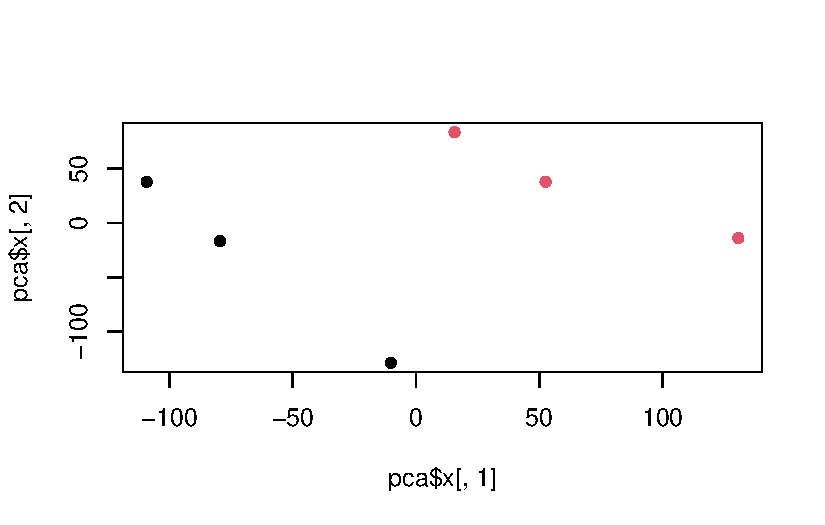
\includegraphics{Class13_files/figure-pdf/unnamed-chunk-7-1.pdf}

}

\end{figure}

\hypertarget{running-deseq2}{%
\section{Running DESeq2}\label{running-deseq2}}

\begin{Shaded}
\begin{Highlighting}[]
\FunctionTok{library}\NormalTok{(DESeq2)}
\end{Highlighting}
\end{Shaded}

\begin{Shaded}
\begin{Highlighting}[]
\NormalTok{dds }\OtherTok{=} \FunctionTok{DESeqDataSetFromMatrix}\NormalTok{(}\AttributeTok{countData=}\NormalTok{counts,}
                             \AttributeTok{colData=}\NormalTok{colData,}
                             \AttributeTok{design=}\SpecialCharTok{\textasciitilde{}}\NormalTok{condition)}
\end{Highlighting}
\end{Shaded}

\begin{verbatim}
Warning in DESeqDataSet(se, design = design, ignoreRank): some variables in
design formula are characters, converting to factors
\end{verbatim}

\begin{Shaded}
\begin{Highlighting}[]
\NormalTok{dds }\OtherTok{=} \FunctionTok{DESeq}\NormalTok{(dds)}
\end{Highlighting}
\end{Shaded}

\begin{verbatim}
estimating size factors
\end{verbatim}

\begin{verbatim}
estimating dispersions
\end{verbatim}

\begin{verbatim}
gene-wise dispersion estimates
\end{verbatim}

\begin{verbatim}
mean-dispersion relationship
\end{verbatim}

\begin{verbatim}
final dispersion estimates
\end{verbatim}

\begin{verbatim}
fitting model and testing
\end{verbatim}

\begin{Shaded}
\begin{Highlighting}[]
\NormalTok{res }\OtherTok{\textless{}{-}} \FunctionTok{results}\NormalTok{(dds)}
\FunctionTok{head}\NormalTok{(res)}
\end{Highlighting}
\end{Shaded}

\begin{verbatim}
log2 fold change (MLE): condition hoxa1 kd vs control sirna 
Wald test p-value: condition hoxa1 kd vs control sirna 
DataFrame with 6 rows and 6 columns
                 baseMean log2FoldChange     lfcSE       stat      pvalue
                <numeric>      <numeric> <numeric>  <numeric>   <numeric>
ENSG00000279457   29.9136      0.1792571 0.3248216   0.551863 5.81042e-01
ENSG00000187634  183.2296      0.4264571 0.1402658   3.040350 2.36304e-03
ENSG00000188976 1651.1881     -0.6927205 0.0548465 -12.630158 1.43990e-36
ENSG00000187961  209.6379      0.7297556 0.1318599   5.534326 3.12428e-08
ENSG00000187583   47.2551      0.0405765 0.2718928   0.149237 8.81366e-01
ENSG00000187642   11.9798      0.5428105 0.5215598   1.040744 2.97994e-01
                       padj
                  <numeric>
ENSG00000279457 6.86555e-01
ENSG00000187634 5.15718e-03
ENSG00000188976 1.76549e-35
ENSG00000187961 1.13413e-07
ENSG00000187583 9.19031e-01
ENSG00000187642 4.03379e-01
\end{verbatim}

\hypertarget{q3}{%
\subsection{\texorpdfstring{\textbf{Q3}}{Q3}}\label{q3}}

\textbf{Call the summary() function on your results to get a sense of
how many genes are up or down-regulated at the default 0.1 p-value
cutoff}

\begin{Shaded}
\begin{Highlighting}[]
\FunctionTok{summary}\NormalTok{(res)}
\end{Highlighting}
\end{Shaded}

\begin{verbatim}

out of 15975 with nonzero total read count
adjusted p-value < 0.1
LFC > 0 (up)       : 4349, 27%
LFC < 0 (down)     : 4396, 28%
outliers [1]       : 0, 0%
low counts [2]     : 1237, 7.7%
(mean count < 0)
[1] see 'cooksCutoff' argument of ?results
[2] see 'independentFiltering' argument of ?results
\end{verbatim}

There are 4349 upregulated genes and 4396 downregulated genes

\begin{Shaded}
\begin{Highlighting}[]
\FunctionTok{plot}\NormalTok{( res}\SpecialCharTok{$}\NormalTok{log2FoldChange, }\SpecialCharTok{{-}}\FunctionTok{log}\NormalTok{(res}\SpecialCharTok{$}\NormalTok{padj) )}
\end{Highlighting}
\end{Shaded}

\begin{figure}[H]

{\centering 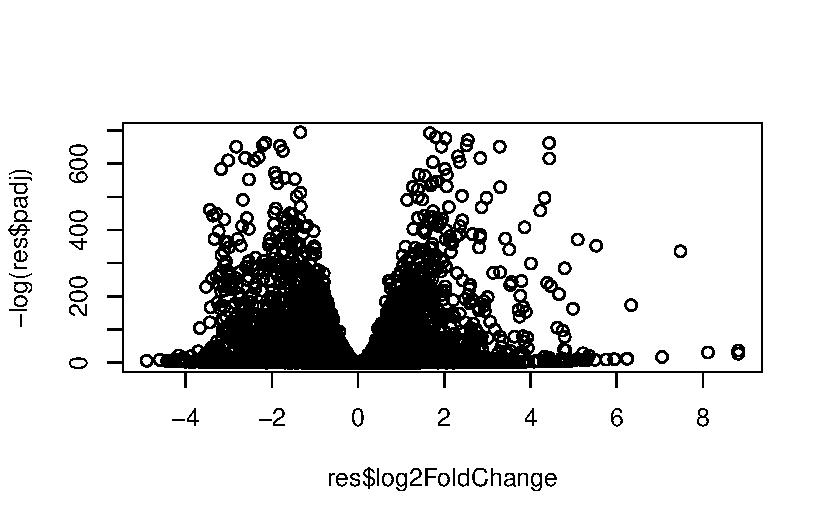
\includegraphics{Class13_files/figure-pdf/unnamed-chunk-11-1.pdf}

}

\end{figure}

\hypertarget{q4}{%
\subsection{\texorpdfstring{\textbf{Q4}}{Q4}}\label{q4}}

\textbf{Improve this plot by completing the below code, which adds color
and axis labels}

\begin{Shaded}
\begin{Highlighting}[]
\CommentTok{\# Make a color vector for all genes}
\NormalTok{mycols }\OtherTok{\textless{}{-}} \FunctionTok{rep}\NormalTok{(}\StringTok{"gray"}\NormalTok{, }\FunctionTok{nrow}\NormalTok{(res) )}

\CommentTok{\# Color red the genes with absolute fold change above 2}
\NormalTok{mycols[res}\SpecialCharTok{$}\NormalTok{log2FoldChange }\SpecialCharTok{\textgreater{}} \DecValTok{2}\NormalTok{ ] }\OtherTok{\textless{}{-}} \StringTok{"blue"}

\CommentTok{\# Color blue those with adjusted p{-}value less than 0.01}
\CommentTok{\#  and absolute fold change more than 2}
\NormalTok{mycols[res}\SpecialCharTok{$}\NormalTok{log2FoldChange }\SpecialCharTok{\textless{}} \SpecialCharTok{{-}}\DecValTok{2}\NormalTok{] }\OtherTok{\textless{}{-}} \StringTok{"red"}
\NormalTok{mycols[res}\SpecialCharTok{$}\NormalTok{padj }\SpecialCharTok{\textgreater{}} \FloatTok{0.05}\NormalTok{ ] }\OtherTok{\textless{}{-}} \StringTok{"green"}

\FunctionTok{plot}\NormalTok{( res}\SpecialCharTok{$}\NormalTok{log2FoldChange, }\SpecialCharTok{{-}}\FunctionTok{log}\NormalTok{(res}\SpecialCharTok{$}\NormalTok{padj), }\AttributeTok{col=}\NormalTok{mycols, }\AttributeTok{xlab=}\StringTok{"Log2(FoldChange)"}\NormalTok{, }\AttributeTok{ylab=}\StringTok{"{-}Log(P{-}value)"}\NormalTok{ )}
\FunctionTok{abline}\NormalTok{(}\AttributeTok{v=}\FunctionTok{c}\NormalTok{(}\SpecialCharTok{{-}}\DecValTok{2}\NormalTok{,}\DecValTok{2}\NormalTok{))}
\end{Highlighting}
\end{Shaded}

\begin{figure}[H]

{\centering 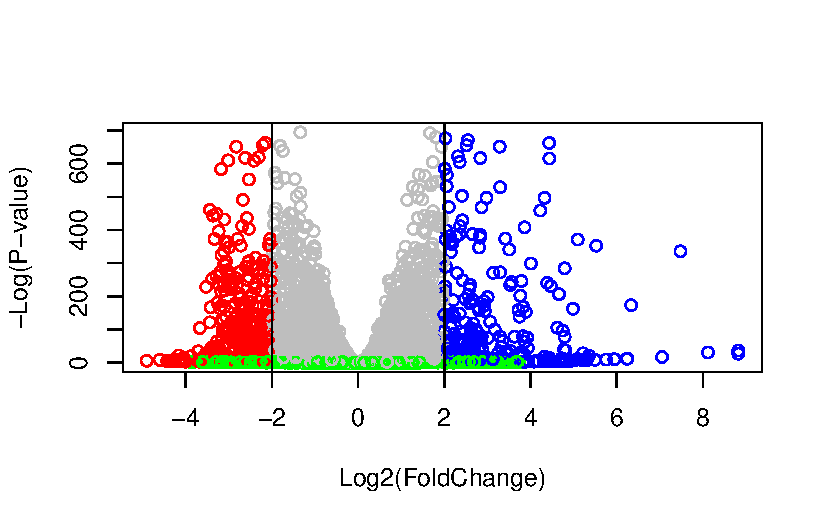
\includegraphics{Class13_files/figure-pdf/unnamed-chunk-12-1.pdf}

}

\end{figure}

\hypertarget{adding-gene-annotation}{%
\section{Adding Gene Annotation}\label{adding-gene-annotation}}

\hypertarget{q5}{%
\subsection{\texorpdfstring{\textbf{Q5}}{Q5}}\label{q5}}

\textbf{Use the mapIDs() function multiple times to add SYMBOL, ENTREZID
and GENENAME annotation to our results by completing the code below.}

\begin{Shaded}
\begin{Highlighting}[]
\FunctionTok{library}\NormalTok{(}\StringTok{"AnnotationDbi"}\NormalTok{)}
\FunctionTok{library}\NormalTok{(}\StringTok{"org.Hs.eg.db"}\NormalTok{)}
\end{Highlighting}
\end{Shaded}

\begin{verbatim}
\end{verbatim}

\begin{Shaded}
\begin{Highlighting}[]
\FunctionTok{columns}\NormalTok{(org.Hs.eg.db)}
\end{Highlighting}
\end{Shaded}

\begin{verbatim}
 [1] "ACCNUM"       "ALIAS"        "ENSEMBL"      "ENSEMBLPROT"  "ENSEMBLTRANS"
 [6] "ENTREZID"     "ENZYME"       "EVIDENCE"     "EVIDENCEALL"  "GENENAME"    
[11] "GENETYPE"     "GO"           "GOALL"        "IPI"          "MAP"         
[16] "OMIM"         "ONTOLOGY"     "ONTOLOGYALL"  "PATH"         "PFAM"        
[21] "PMID"         "PROSITE"      "REFSEQ"       "SYMBOL"       "UCSCKG"      
[26] "UNIPROT"     
\end{verbatim}

\begin{Shaded}
\begin{Highlighting}[]
\NormalTok{res}\SpecialCharTok{$}\NormalTok{symbol }\OtherTok{\textless{}{-}}  \FunctionTok{mapIds}\NormalTok{(org.Hs.eg.db,}
                    \AttributeTok{keys=}\FunctionTok{row.names}\NormalTok{(res), }
                    \AttributeTok{keytype=}\StringTok{"ENSEMBL"}\NormalTok{,}
                    \AttributeTok{column=}\StringTok{"SYMBOL"}\NormalTok{,}
                    \AttributeTok{multiVals=}\StringTok{"first"}\NormalTok{)}
\end{Highlighting}
\end{Shaded}

\begin{verbatim}
'select()' returned 1:many mapping between keys and columns
\end{verbatim}

\begin{Shaded}
\begin{Highlighting}[]
\NormalTok{res}\SpecialCharTok{$}\NormalTok{entrez }\OtherTok{\textless{}{-}}  \FunctionTok{mapIds}\NormalTok{(org.Hs.eg.db,}
                    \AttributeTok{keys=}\FunctionTok{row.names}\NormalTok{(res),}
                    \AttributeTok{keytype=}\StringTok{"ENSEMBL"}\NormalTok{,}
                    \AttributeTok{column=}\StringTok{"ENTREZID"}\NormalTok{,}
                    \AttributeTok{multiVals=}\StringTok{"first"}\NormalTok{)}
\end{Highlighting}
\end{Shaded}

\begin{verbatim}
'select()' returned 1:many mapping between keys and columns
\end{verbatim}

\begin{Shaded}
\begin{Highlighting}[]
\NormalTok{res}\SpecialCharTok{$}\NormalTok{name }\OtherTok{\textless{}{-}}  \FunctionTok{mapIds}\NormalTok{(org.Hs.eg.db,}
                    \AttributeTok{keys=}\FunctionTok{row.names}\NormalTok{(res),}
                    \AttributeTok{keytype=}\StringTok{"ENSEMBL"}\NormalTok{,}
                    \AttributeTok{column=}\StringTok{"GENENAME"}\NormalTok{,}
                    \AttributeTok{multiVals=}\StringTok{"first"}\NormalTok{)}
\end{Highlighting}
\end{Shaded}

\begin{verbatim}
'select()' returned 1:many mapping between keys and columns
\end{verbatim}

\begin{Shaded}
\begin{Highlighting}[]
\FunctionTok{head}\NormalTok{(res, }\DecValTok{10}\NormalTok{)}
\end{Highlighting}
\end{Shaded}

\begin{verbatim}
log2 fold change (MLE): condition hoxa1 kd vs control sirna 
Wald test p-value: condition hoxa1 kd vs control sirna 
DataFrame with 10 rows and 9 columns
                   baseMean log2FoldChange     lfcSE       stat      pvalue
                  <numeric>      <numeric> <numeric>  <numeric>   <numeric>
ENSG00000279457   29.913579      0.1792571 0.3248216   0.551863 5.81042e-01
ENSG00000187634  183.229650      0.4264571 0.1402658   3.040350 2.36304e-03
ENSG00000188976 1651.188076     -0.6927205 0.0548465 -12.630158 1.43990e-36
ENSG00000187961  209.637938      0.7297556 0.1318599   5.534326 3.12428e-08
ENSG00000187583   47.255123      0.0405765 0.2718928   0.149237 8.81366e-01
ENSG00000187642   11.979750      0.5428105 0.5215598   1.040744 2.97994e-01
ENSG00000188290  108.922128      2.0570638 0.1969053  10.446970 1.51282e-25
ENSG00000187608  350.716868      0.2573837 0.1027266   2.505522 1.22271e-02
ENSG00000188157 9128.439422      0.3899088 0.0467163   8.346304 7.04321e-17
ENSG00000237330    0.158192      0.7859552 4.0804729   0.192614 8.47261e-01
                       padj      symbol      entrez                   name
                  <numeric> <character> <character>            <character>
ENSG00000279457 6.86555e-01          NA          NA                     NA
ENSG00000187634 5.15718e-03      SAMD11      148398 sterile alpha motif ..
ENSG00000188976 1.76549e-35       NOC2L       26155 NOC2 like nucleolar ..
ENSG00000187961 1.13413e-07      KLHL17      339451 kelch like family me..
ENSG00000187583 9.19031e-01     PLEKHN1       84069 pleckstrin homology ..
ENSG00000187642 4.03379e-01       PERM1       84808 PPARGC1 and ESRR ind..
ENSG00000188290 1.30538e-24        HES4       57801 hes family bHLH tran..
ENSG00000187608 2.37452e-02       ISG15        9636 ISG15 ubiquitin like..
ENSG00000188157 4.21963e-16        AGRN      375790                  agrin
ENSG00000237330          NA      RNF223      401934 ring finger protein ..
\end{verbatim}

\hypertarget{q6}{%
\subsection{\texorpdfstring{\textbf{Q6}}{Q6}}\label{q6}}

\textbf{Finally for this section let's reorder these results by adjusted
p-value and save them to a CSV file in your current project directory.}

\begin{Shaded}
\begin{Highlighting}[]
\NormalTok{res }\OtherTok{=}\NormalTok{ res[}\FunctionTok{order}\NormalTok{(res}\SpecialCharTok{$}\NormalTok{pvalue),]}
\FunctionTok{write.csv}\NormalTok{(res, }\AttributeTok{file=}\StringTok{"deseq\_results.csv"}\NormalTok{)}
\end{Highlighting}
\end{Shaded}

\hypertarget{section-2-pathway-analysis-or-gene-set-enrichment}{%
\section{Section 2: Pathway Analysis or Gene Set
Enrichment}\label{section-2-pathway-analysis-or-gene-set-enrichment}}

We can use \texttt{gage()} with KEGG and GO

\begin{Shaded}
\begin{Highlighting}[]
\FunctionTok{library}\NormalTok{(gage)}
\FunctionTok{library}\NormalTok{(gageData)}
\FunctionTok{library}\NormalTok{(pathview)}

\FunctionTok{data}\NormalTok{(kegg.sets.hs)}
\FunctionTok{data}\NormalTok{(sigmet.idx.hs)}

\CommentTok{\# Focus on signaling and metabolic pathways only}
\NormalTok{kegg.sets.hs }\OtherTok{=}\NormalTok{ kegg.sets.hs[sigmet.idx.hs]}

\CommentTok{\# Examine the first 3 pathways}
\FunctionTok{head}\NormalTok{(kegg.sets.hs, }\DecValTok{3}\NormalTok{)}
\end{Highlighting}
\end{Shaded}

\begin{verbatim}
$`hsa00232 Caffeine metabolism`
[1] "10"   "1544" "1548" "1549" "1553" "7498" "9"   

$`hsa00983 Drug metabolism - other enzymes`
 [1] "10"     "1066"   "10720"  "10941"  "151531" "1548"   "1549"   "1551"  
 [9] "1553"   "1576"   "1577"   "1806"   "1807"   "1890"   "221223" "2990"  
[17] "3251"   "3614"   "3615"   "3704"   "51733"  "54490"  "54575"  "54576" 
[25] "54577"  "54578"  "54579"  "54600"  "54657"  "54658"  "54659"  "54963" 
[33] "574537" "64816"  "7083"   "7084"   "7172"   "7363"   "7364"   "7365"  
[41] "7366"   "7367"   "7371"   "7372"   "7378"   "7498"   "79799"  "83549" 
[49] "8824"   "8833"   "9"      "978"   

$`hsa00230 Purine metabolism`
  [1] "100"    "10201"  "10606"  "10621"  "10622"  "10623"  "107"    "10714" 
  [9] "108"    "10846"  "109"    "111"    "11128"  "11164"  "112"    "113"   
 [17] "114"    "115"    "122481" "122622" "124583" "132"    "158"    "159"   
 [25] "1633"   "171568" "1716"   "196883" "203"    "204"    "205"    "221823"
 [33] "2272"   "22978"  "23649"  "246721" "25885"  "2618"   "26289"  "270"   
 [41] "271"    "27115"  "272"    "2766"   "2977"   "2982"   "2983"   "2984"  
 [49] "2986"   "2987"   "29922"  "3000"   "30833"  "30834"  "318"    "3251"  
 [57] "353"    "3614"   "3615"   "3704"   "377841" "471"    "4830"   "4831"  
 [65] "4832"   "4833"   "4860"   "4881"   "4882"   "4907"   "50484"  "50940" 
 [73] "51082"  "51251"  "51292"  "5136"   "5137"   "5138"   "5139"   "5140"  
 [81] "5141"   "5142"   "5143"   "5144"   "5145"   "5146"   "5147"   "5148"  
 [89] "5149"   "5150"   "5151"   "5152"   "5153"   "5158"   "5167"   "5169"  
 [97] "51728"  "5198"   "5236"   "5313"   "5315"   "53343"  "54107"  "5422"  
[105] "5424"   "5425"   "5426"   "5427"   "5430"   "5431"   "5432"   "5433"  
[113] "5434"   "5435"   "5436"   "5437"   "5438"   "5439"   "5440"   "5441"  
[121] "5471"   "548644" "55276"  "5557"   "5558"   "55703"  "55811"  "55821" 
[129] "5631"   "5634"   "56655"  "56953"  "56985"  "57804"  "58497"  "6240"  
[137] "6241"   "64425"  "646625" "654364" "661"    "7498"   "8382"   "84172" 
[145] "84265"  "84284"  "84618"  "8622"   "8654"   "87178"  "8833"   "9060"  
[153] "9061"   "93034"  "953"    "9533"   "954"    "955"    "956"    "957"   
[161] "9583"   "9615"  
\end{verbatim}

\begin{Shaded}
\begin{Highlighting}[]
\NormalTok{foldchanges }\OtherTok{=}\NormalTok{ res}\SpecialCharTok{$}\NormalTok{log2FoldChange}
\FunctionTok{names}\NormalTok{(foldchanges) }\OtherTok{=}\NormalTok{ res}\SpecialCharTok{$}\NormalTok{entrez}
\FunctionTok{head}\NormalTok{(foldchanges)}
\end{Highlighting}
\end{Shaded}

\begin{verbatim}
     1266     54855      1465     51232      2034      2317 
-2.422719  3.201955 -2.313738 -2.059631 -1.888019 -1.649792 
\end{verbatim}

\begin{Shaded}
\begin{Highlighting}[]
\NormalTok{keggres }\OtherTok{=} \FunctionTok{gage}\NormalTok{(foldchanges, }\AttributeTok{gsets=}\NormalTok{kegg.sets.hs)}
\FunctionTok{attributes}\NormalTok{(keggres)}
\end{Highlighting}
\end{Shaded}

\begin{verbatim}
$names
[1] "greater" "less"    "stats"  
\end{verbatim}

\begin{Shaded}
\begin{Highlighting}[]
\FunctionTok{head}\NormalTok{(keggres}\SpecialCharTok{$}\NormalTok{less)}
\end{Highlighting}
\end{Shaded}

\begin{verbatim}
                                         p.geomean stat.mean        p.val
hsa04110 Cell cycle                   8.995727e-06 -4.378644 8.995727e-06
hsa03030 DNA replication              9.424076e-05 -3.951803 9.424076e-05
hsa03013 RNA transport                1.375901e-03 -3.028500 1.375901e-03
hsa03440 Homologous recombination     3.066756e-03 -2.852899 3.066756e-03
hsa04114 Oocyte meiosis               3.784520e-03 -2.698128 3.784520e-03
hsa00010 Glycolysis / Gluconeogenesis 8.961413e-03 -2.405398 8.961413e-03
                                            q.val set.size         exp1
hsa04110 Cell cycle                   0.001448312      121 8.995727e-06
hsa03030 DNA replication              0.007586381       36 9.424076e-05
hsa03013 RNA transport                0.073840037      144 1.375901e-03
hsa03440 Homologous recombination     0.121861535       28 3.066756e-03
hsa04114 Oocyte meiosis               0.121861535      102 3.784520e-03
hsa00010 Glycolysis / Gluconeogenesis 0.212222694       53 8.961413e-03
\end{verbatim}

\begin{Shaded}
\begin{Highlighting}[]
\FunctionTok{pathview}\NormalTok{(}\AttributeTok{gene.data=}\NormalTok{foldchanges, }\AttributeTok{pathway.id=}\StringTok{"hsa04110"}\NormalTok{)}
\end{Highlighting}
\end{Shaded}

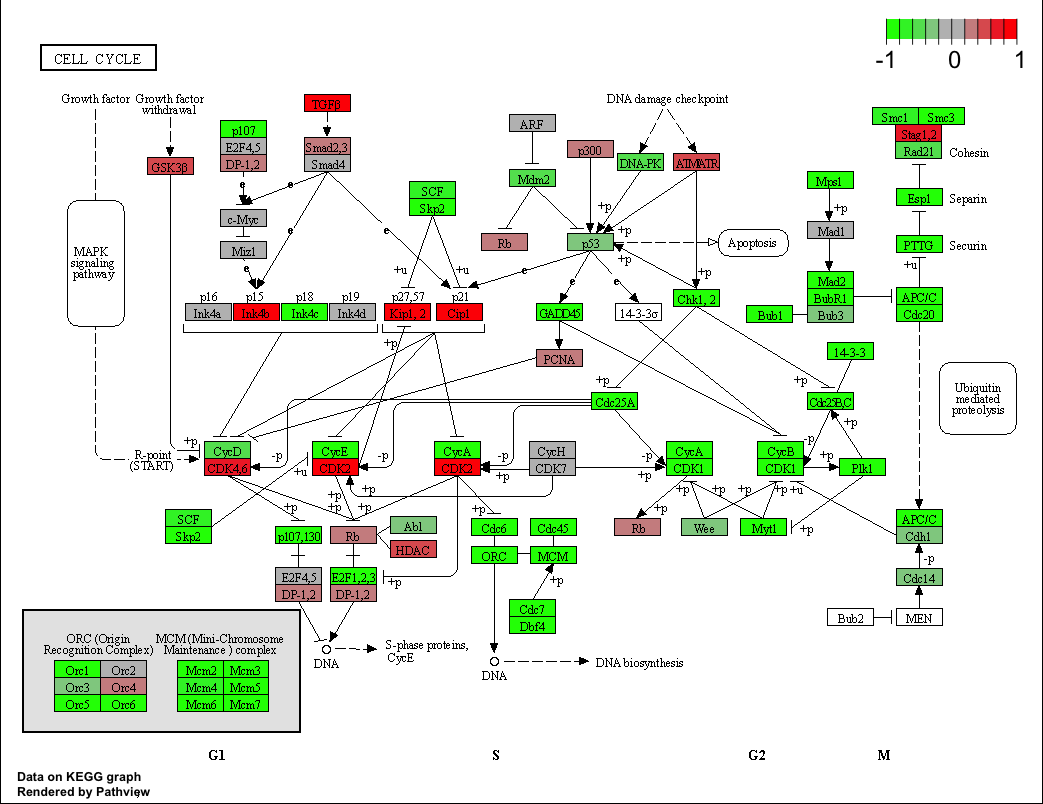
\includegraphics{hsa04110.pathview.png}

\begin{Shaded}
\begin{Highlighting}[]
\DocumentationTok{\#\# Focus on top 5 upregulated pathways here for demo purposes only}
\NormalTok{keggrespathways }\OtherTok{\textless{}{-}} \FunctionTok{rownames}\NormalTok{(keggres}\SpecialCharTok{$}\NormalTok{greater)[}\DecValTok{1}\SpecialCharTok{:}\DecValTok{5}\NormalTok{]}

\CommentTok{\# Extract the 8 character long IDs part of each string}
\NormalTok{keggresids }\OtherTok{=} \FunctionTok{substr}\NormalTok{(keggrespathways, }\AttributeTok{start=}\DecValTok{1}\NormalTok{, }\AttributeTok{stop=}\DecValTok{8}\NormalTok{)}
\NormalTok{keggresids}
\end{Highlighting}
\end{Shaded}

\begin{verbatim}
[1] "hsa04640" "hsa04630" "hsa00140" "hsa04142" "hsa04330"
\end{verbatim}

\begin{Shaded}
\begin{Highlighting}[]
\FunctionTok{pathview}\NormalTok{(}\AttributeTok{gene.data=}\NormalTok{foldchanges, }\AttributeTok{pathway.id=}\NormalTok{keggresids, }\AttributeTok{species=}\StringTok{"hsa"}\NormalTok{)}
\end{Highlighting}
\end{Shaded}

\hypertarget{q7}{%
\subsection{\texorpdfstring{\textbf{Q7}}{Q7}}\label{q7}}

\textbf{Can you do the same procedure as above to plot the pathview
figures for the top 5 down-reguled pathways?}

\begin{Shaded}
\begin{Highlighting}[]
\DocumentationTok{\#\# Focus on top 5 downregulated pathways here for demo purposes only}
\NormalTok{keggrespathways\_down }\OtherTok{\textless{}{-}} \FunctionTok{rownames}\NormalTok{(keggres}\SpecialCharTok{$}\NormalTok{less)[}\DecValTok{1}\SpecialCharTok{:}\DecValTok{5}\NormalTok{]}

\CommentTok{\# Extract the 8 character long IDs part of each string}
\NormalTok{keggresids\_down }\OtherTok{=} \FunctionTok{substr}\NormalTok{(keggrespathways\_down, }\AttributeTok{start=}\DecValTok{1}\NormalTok{, }\AttributeTok{stop=}\DecValTok{8}\NormalTok{)}
\NormalTok{keggresids\_down}
\end{Highlighting}
\end{Shaded}

\begin{verbatim}
[1] "hsa04110" "hsa03030" "hsa03013" "hsa03440" "hsa04114"
\end{verbatim}

\begin{Shaded}
\begin{Highlighting}[]
\FunctionTok{pathview}\NormalTok{(}\AttributeTok{gene.data=}\NormalTok{foldchanges, }\AttributeTok{pathway.id=}\NormalTok{keggresids, }\AttributeTok{species=}\StringTok{"hsa"}\NormalTok{)}
\end{Highlighting}
\end{Shaded}

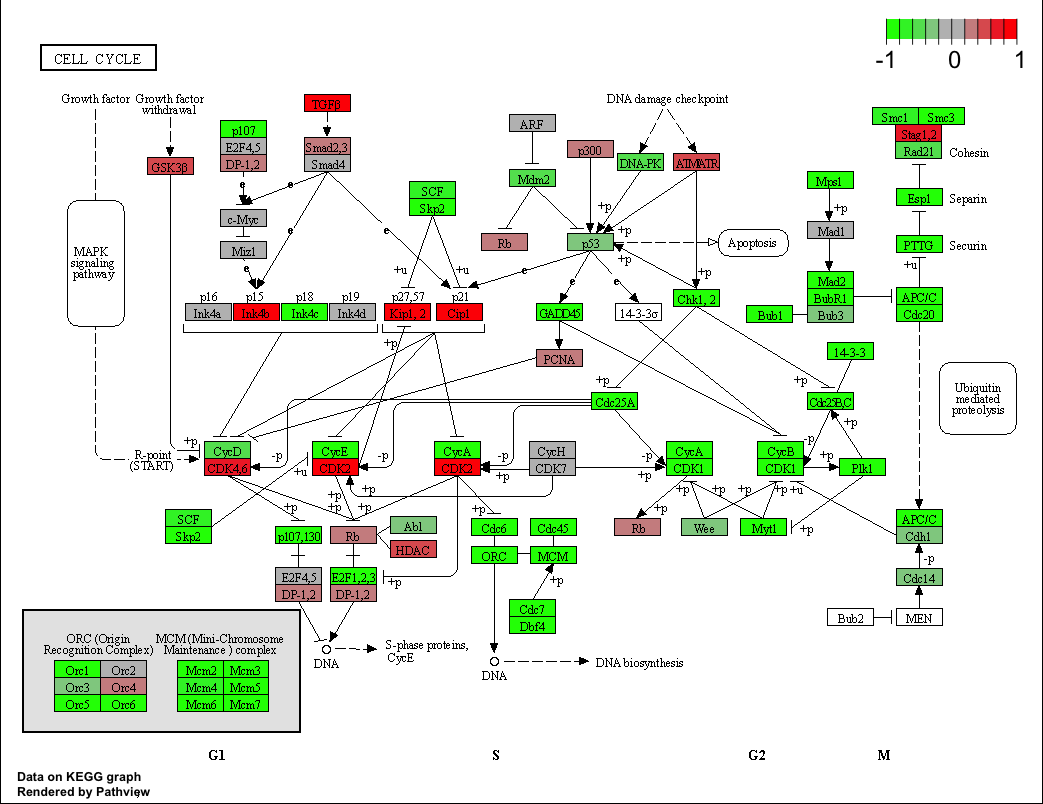
\includegraphics{hsa04110.pathview.png}
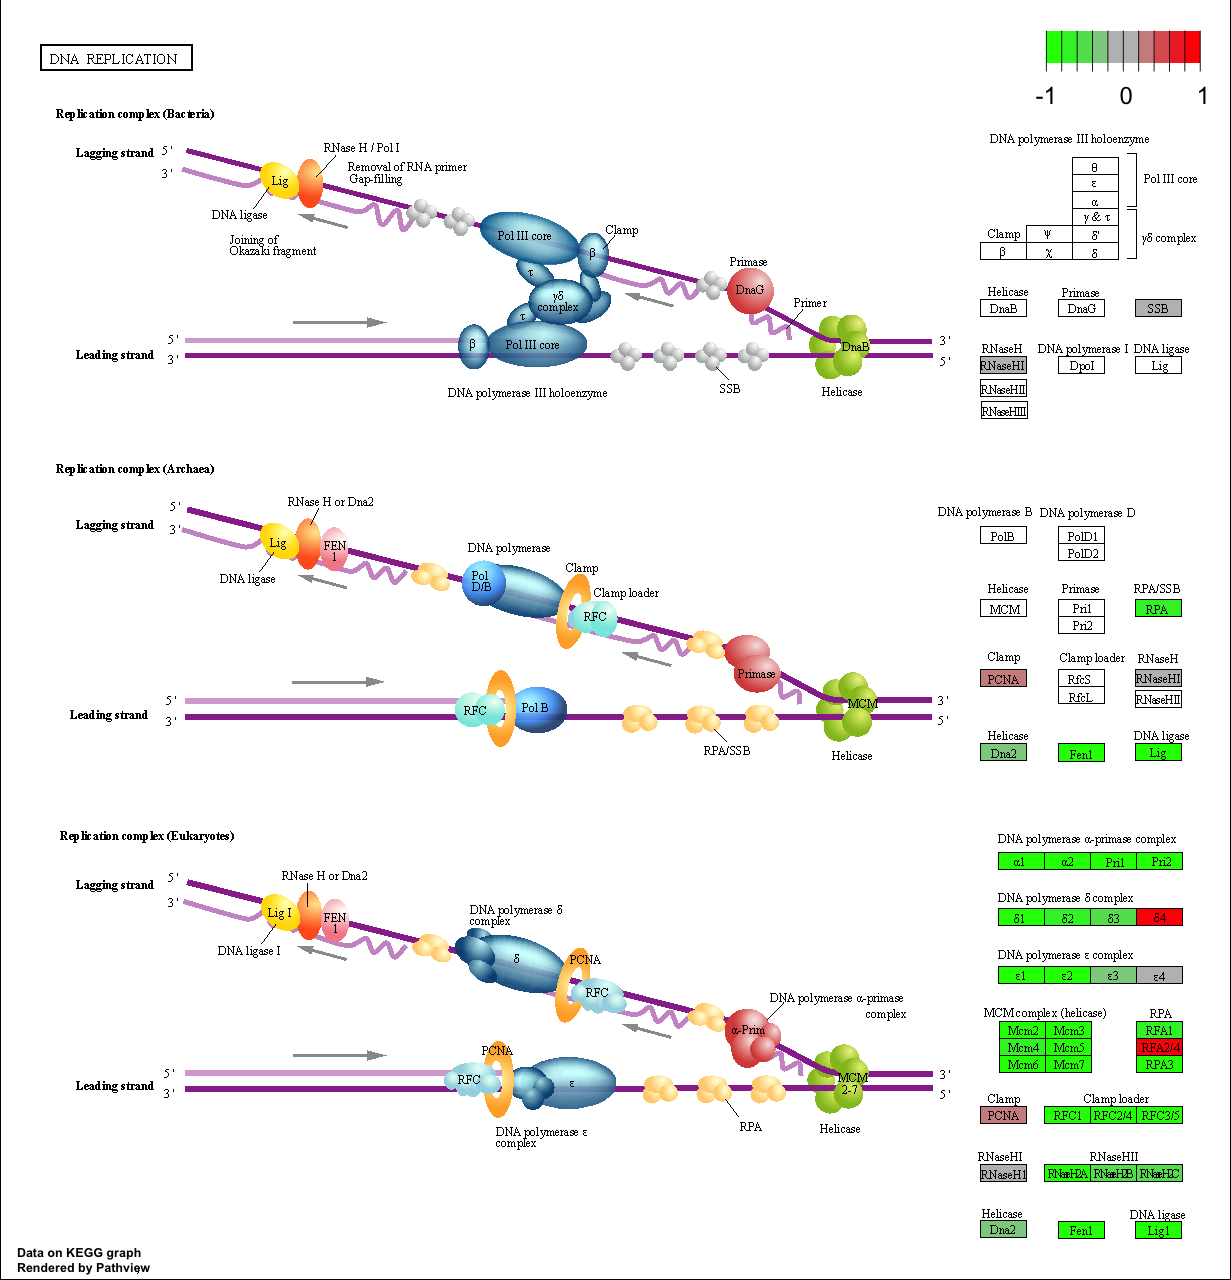
\includegraphics{hsa03030.pathview.png}
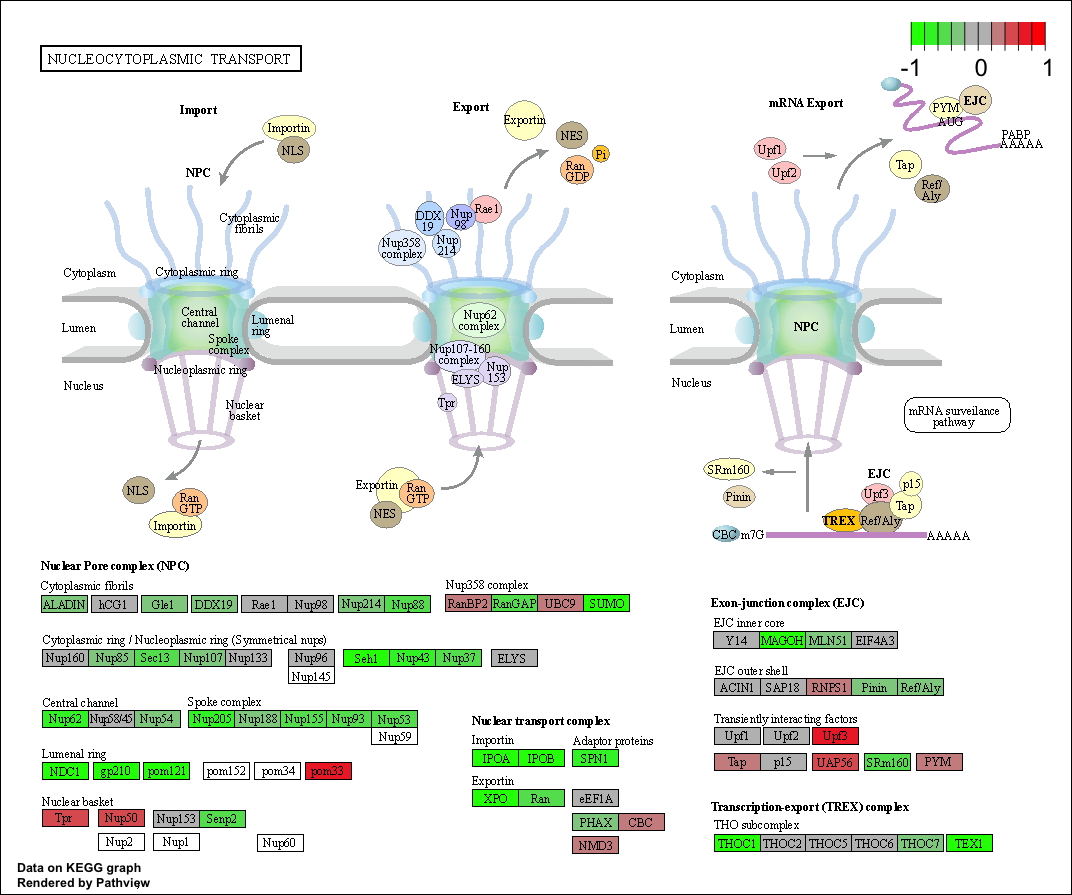
\includegraphics{hsa03013.pathview.png}
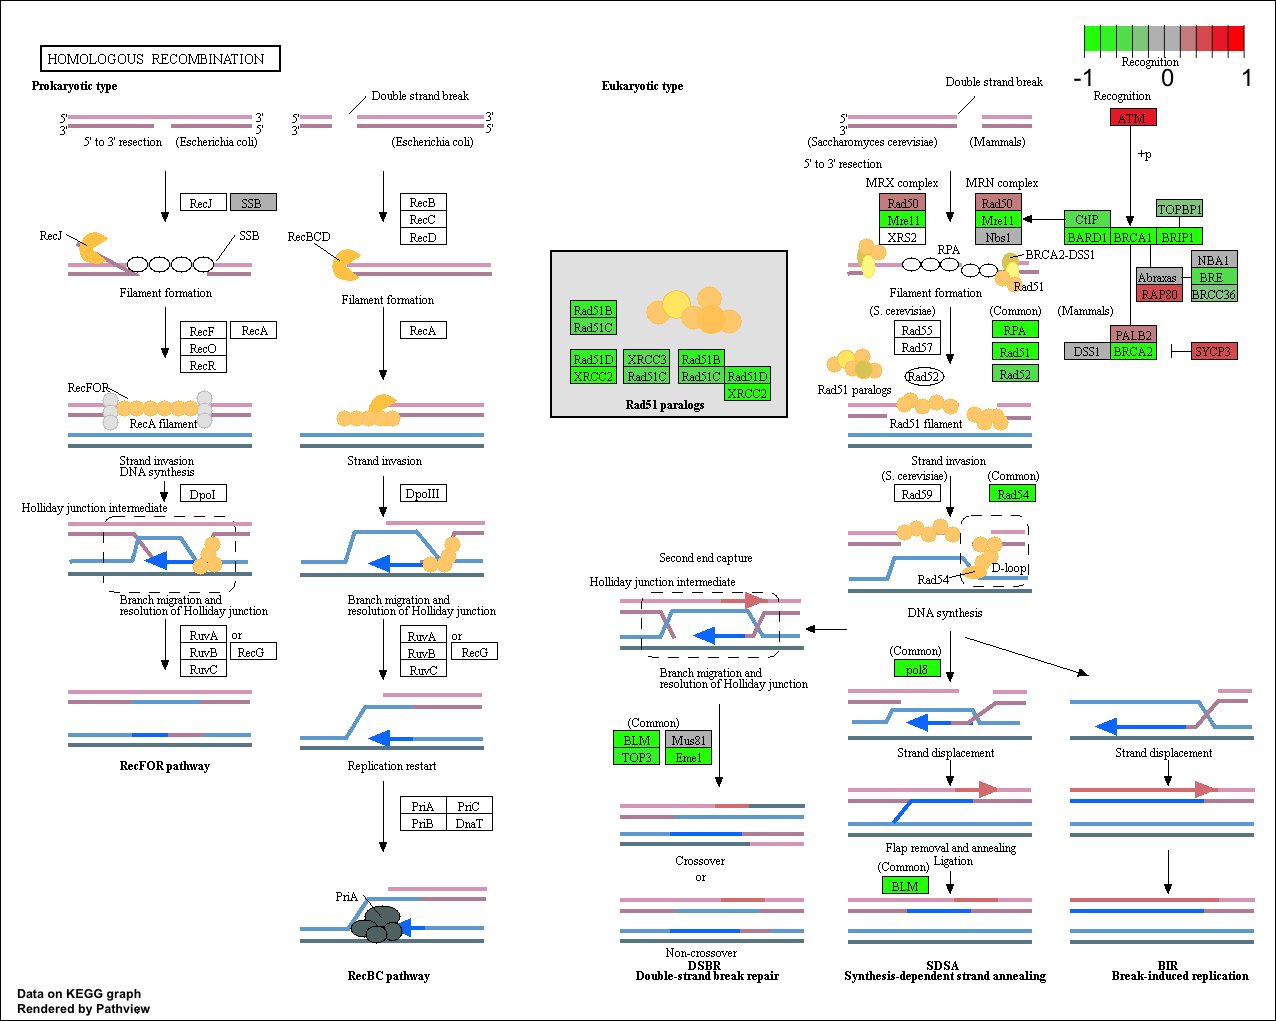
\includegraphics{hsa03440.pathview.png}
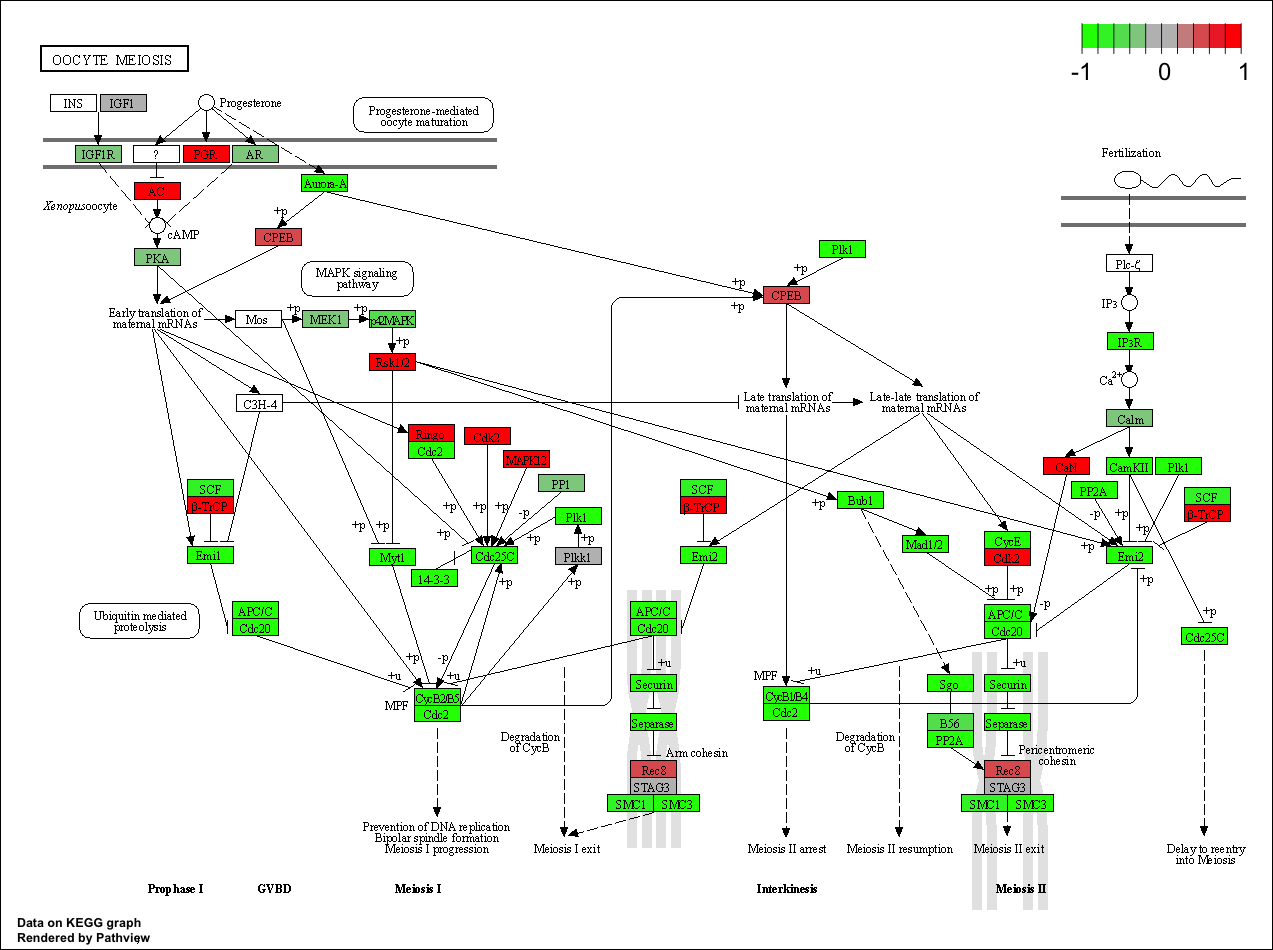
\includegraphics{hsa04114.pathview.png}

\hypertarget{section-3-gene-ontology}{%
\section{Section 3: Gene Ontology}\label{section-3-gene-ontology}}

\begin{Shaded}
\begin{Highlighting}[]
\FunctionTok{data}\NormalTok{(go.sets.hs)}
\FunctionTok{data}\NormalTok{(go.subs.hs)}

\CommentTok{\# Focus on Biological Process subset of GO}
\NormalTok{gobpsets }\OtherTok{=}\NormalTok{ go.sets.hs[go.subs.hs}\SpecialCharTok{$}\NormalTok{BP]}

\NormalTok{gobpres }\OtherTok{=} \FunctionTok{gage}\NormalTok{(foldchanges, }\AttributeTok{gsets=}\NormalTok{gobpsets, }\AttributeTok{same.dir=}\ConstantTok{TRUE}\NormalTok{)}

\FunctionTok{lapply}\NormalTok{(gobpres, head)}
\end{Highlighting}
\end{Shaded}

\begin{verbatim}
$greater
                                             p.geomean stat.mean        p.val
GO:0007156 homophilic cell adhesion       8.519724e-05  3.824205 8.519724e-05
GO:0002009 morphogenesis of an epithelium 1.396681e-04  3.653886 1.396681e-04
GO:0048729 tissue morphogenesis           1.432451e-04  3.643242 1.432451e-04
GO:0007610 behavior                       2.195494e-04  3.530241 2.195494e-04
GO:0060562 epithelial tube morphogenesis  5.932837e-04  3.261376 5.932837e-04
GO:0035295 tube development               5.953254e-04  3.253665 5.953254e-04
                                              q.val set.size         exp1
GO:0007156 homophilic cell adhesion       0.1951953      113 8.519724e-05
GO:0002009 morphogenesis of an epithelium 0.1951953      339 1.396681e-04
GO:0048729 tissue morphogenesis           0.1951953      424 1.432451e-04
GO:0007610 behavior                       0.2243795      427 2.195494e-04
GO:0060562 epithelial tube morphogenesis  0.3711390      257 5.932837e-04
GO:0035295 tube development               0.3711390      391 5.953254e-04

$less
                                            p.geomean stat.mean        p.val
GO:0048285 organelle fission             1.536227e-15 -8.063910 1.536227e-15
GO:0000280 nuclear division              4.286961e-15 -7.939217 4.286961e-15
GO:0007067 mitosis                       4.286961e-15 -7.939217 4.286961e-15
GO:0000087 M phase of mitotic cell cycle 1.169934e-14 -7.797496 1.169934e-14
GO:0007059 chromosome segregation        2.028624e-11 -6.878340 2.028624e-11
GO:0000236 mitotic prometaphase          1.729553e-10 -6.695966 1.729553e-10
                                                q.val set.size         exp1
GO:0048285 organelle fission             5.841698e-12      376 1.536227e-15
GO:0000280 nuclear division              5.841698e-12      352 4.286961e-15
GO:0007067 mitosis                       5.841698e-12      352 4.286961e-15
GO:0000087 M phase of mitotic cell cycle 1.195672e-11      362 1.169934e-14
GO:0007059 chromosome segregation        1.658603e-08      142 2.028624e-11
GO:0000236 mitotic prometaphase          1.178402e-07       84 1.729553e-10

$stats
                                          stat.mean     exp1
GO:0007156 homophilic cell adhesion        3.824205 3.824205
GO:0002009 morphogenesis of an epithelium  3.653886 3.653886
GO:0048729 tissue morphogenesis            3.643242 3.643242
GO:0007610 behavior                        3.530241 3.530241
GO:0060562 epithelial tube morphogenesis   3.261376 3.261376
GO:0035295 tube development                3.253665 3.253665
\end{verbatim}

\hypertarget{section-4-reactome-analysis}{%
\section{Section 4: Reactome
Analysis}\label{section-4-reactome-analysis}}

\begin{Shaded}
\begin{Highlighting}[]
\NormalTok{sig\_genes }\OtherTok{\textless{}{-}}\NormalTok{ res[res}\SpecialCharTok{$}\NormalTok{padj }\SpecialCharTok{\textless{}=} \FloatTok{0.05} \SpecialCharTok{\&} \SpecialCharTok{!}\FunctionTok{is.na}\NormalTok{(res}\SpecialCharTok{$}\NormalTok{padj), }\StringTok{"symbol"}\NormalTok{]}
\FunctionTok{print}\NormalTok{(}\FunctionTok{paste}\NormalTok{(}\StringTok{"Total number of significant genes:"}\NormalTok{, }\FunctionTok{length}\NormalTok{(sig\_genes)))}
\end{Highlighting}
\end{Shaded}

\begin{verbatim}
[1] "Total number of significant genes: 8147"
\end{verbatim}

\begin{Shaded}
\begin{Highlighting}[]
\FunctionTok{write.table}\NormalTok{(sig\_genes, }\AttributeTok{file=}\StringTok{"significant\_genes.txt"}\NormalTok{, }\AttributeTok{row.names=}\ConstantTok{FALSE}\NormalTok{, }\AttributeTok{col.names=}\ConstantTok{FALSE}\NormalTok{, }\AttributeTok{quote=}\ConstantTok{FALSE}\NormalTok{)}
\end{Highlighting}
\end{Shaded}

\hypertarget{q8}{%
\subsection{\texorpdfstring{\textbf{Q8}}{Q8}}\label{q8}}

\textbf{What pathway has the most significant ``Entities p-value''? Do
the most significant pathways listed match your previous KEGG results?
What factors could cause differences between the two methods?}

The most significant Entities p-value is the Endosomal/ Vacuolar
Pathway. The most significant pathways do not match the KEGG results.
The likely difference between these results are because they are built
from 2 separate databases.



\end{document}
